\section{总结与体会}

这次project给我的帮助主要有两点: 学习了新的算法和认识到了测试的重要性。

完成这个Project大概花了我两个星期时间,其中确立思路与框架花了一天,写程序花了两天,剩下的时间都用于调试与测试数据。以前我对测试的重要性有所忽视,总认为反正程序很短,运用中可以出了问题再改。但是这次的工程量略微上升了一点,这种方法的弊病就出现了。对于一个表达式而言,需要考虑的corner case非常多。如果程序不能有一个很好的架构的话,很难考虑到所有情况,调试将会变得非常麻烦。因此,程序的合理组织比正确的写出程序更加重要。

而就这个project而言,它需要的两个函数expr$\_$to$\_$truthtable和truthtable$\_$to$\_$expr,我分别用了两个类ExpressionToChart和ChartToExpression来完成,而在ChartToExpression中,针对质蕴涵项这个概念被多次使用的情况,又另见了$implication$类来专门实现质蕴涵的相关操作。这样,这个project的架构就比较清晰,也比较利于调试了。

当然,这次project让我学习了Q-M算法和petrick化简,同时也复习了表达式求值这以经典算法。在实现上来说,表达式求值相对易于实现,因此expr$\_$to$\_$truthtable这个函数实现的较为轻松。而Q-M算法是我较为陌生的一种算法,较为繁琐。我在实现时也遇到了一些困难,但主要是由于我对于算法不太熟悉,思路不够清晰。经过几次的重构,这一部分才算完成。《孙子兵法》中说:“谋定而后动,知止而有得”。对于一个工程来说,要时刻保持思路的清晰,这比纯粹的垒代码重要的多。

很惭愧,就做了一点微小的工作。Linus Torvalds说过:“Talk is cheap, show me the code.”希望以这次的Mini$\_$Project作为起步,通过期末的Final$\_$Project,在实践中不断提示自己的工程能力。

\vspace{2cm}

\begin{figure}[h]
	\centering
		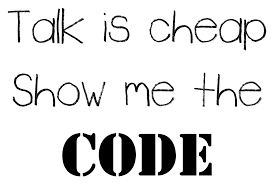
\includegraphics[scale=0.8]{images/linus.png}
\end{figure}